\documentclass[]{article}
\usepackage[margin=1.25in]{geometry}
\usepackage{graphicx}
\graphicspath{ {./images/} }
\usepackage{float}

\usepackage[bibstyle=apa, sorting=nyt, backend=biber, citestyle=authoryear, natbib]{biblatex}
\addbibresource{refs.bib}

\title{Honk Honk}
\author{Aden Northcote}
\date{}


\begin{document}
    
\maketitle

\tableofcontents

\clearpage

\section{Background}

SmartV is a popular online platform providing a wide range of video tools to end-users. Services are provided to consumers over the internet and include video streaming and delivery, video searching, video editing, video transcoding and adaptation.

The SmartV platform is well used and is currently experiencing significant growth in user-base. This trend has prompted a transition from on-premises infrastructure to the cloud with the aim of future-proofing the company's scalability and cost-competitiveness.

\section{Business Requirements}

The operating model of the SmartV platform relies heavily on ready access to large amounts of storage, compute, and networking capability. This is especially true given the large amounts of high resolution video data the platform is expected to process and store. The business requirements captured from this understanding are presented here in two sections: the requirements relating to SmartV's operations and the requirements relating to the cloud infrastructure specifically.

\subsection{Operational Requirements}

\subsubsection{Scalability}

Scalability represents a primary business objective for SmartV's transition to cloud-based infrastructure, and underlies most of the business requirements outlined in this document. The deployment of scalable infrastructure provides SmartV the ability to react to fluctuations in platform usage while minimising any costs associated with under-utilised infrastructure.

\subsubsection{Availability}

The SmartV platform's customer-facing model requires services to be highly available to end-users, ensuring uninterrupted access to videos and features. Services need to be available even during peak usage times or unforeseen spikes in demand.

% S3 has 4 9's of durability https://docs.aws.amazon.com/AmazonS3/latest/userguide/DataDurability.html

\subsubsection{Reliability}

The cloud infrastructure used to enable SmartV must also prioritise high availability, with resilient architecture that minimises downtime and ensures continuous service delivery. 

\subsection{Infrastructure Requirements}

% S3 has 11 9's of durability 

\subsection{Storage}

Effective storage management is a key requirement of SmartV's infrastructure, with the service housing massive amounts of video data for its users. A viable storage solution for the transition to cloud must fulfil the following:

\begin{description}
    \item[Scalable] As SmartV's user base continues to grow, a viable storage solution must be able to cope with fluctuations in storage requirements.
    \item[Reliable] The storage implementation provided to SmartV must provide hosted files to users reliably.
    \item[High Availability] SmartV hosted files must be highly available to users, with built in redundancy measures.
\end{description}



\subsection{Compute}

The computational intensity of video based workloads necessitates significant amounts of domain-specific compute availability in the form of graphics processing unit (GPU) access, as well as the additional components required to support them. 

\begin{description}
    \item[] description
\end{description}

\subsection{Network}

\subsection{Availability}

\subsection{Security}

\subsection{Infrastructure Management}

\subsection{Other stuff DELETE}
`` Some other basic cloud implementation/management requirements, such as high availability, DRS,
resource control, updating, etc. ''

\section{Cloud Architecture and Design}

\subsection{Platform Selection}



\subsection{Design Assumptions}

\subsection{Infrastructure Design}
\begin{figure}[H]\label{fig:awsdiagram}
    \centering
    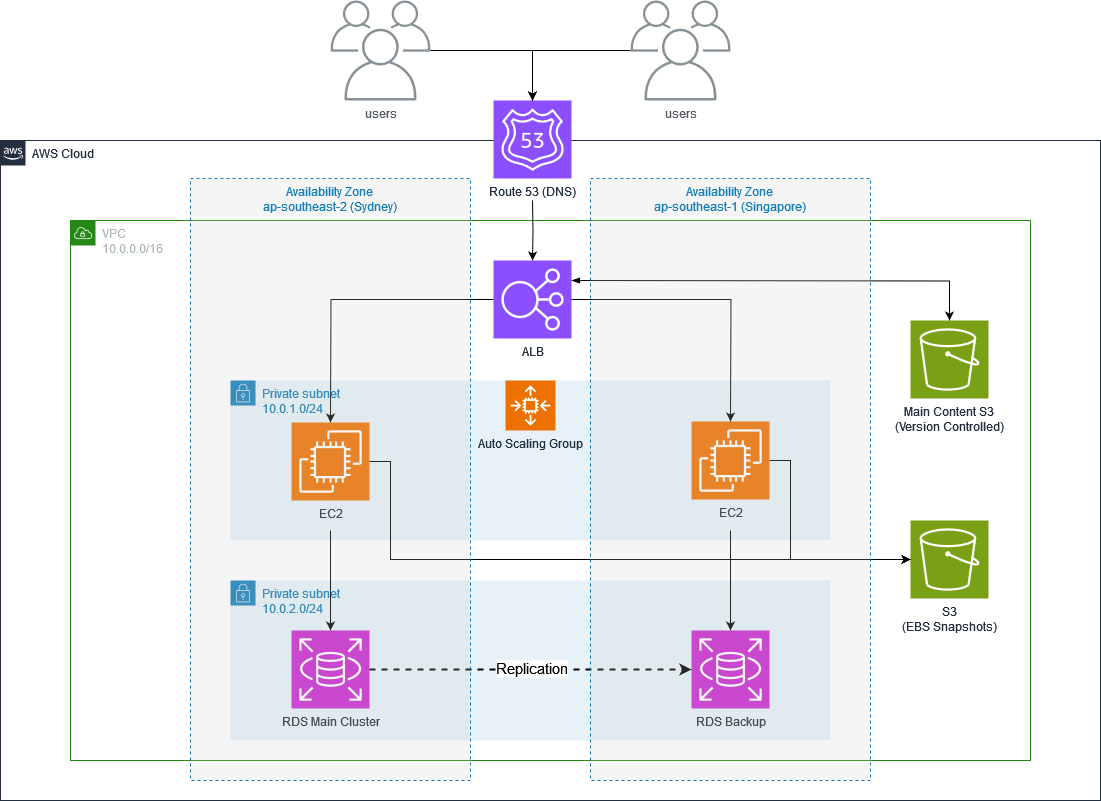
\includegraphics[width=\textwidth]{cci_aws}
    \caption{Cloud Infrastructure Topology}
\end{figure}

\subsection{Pricing}

% https://calculator.aws/#/addService

\section{Considerations and Challenges}

\section{Evolution of Technology}



\end{document}